\documentclass[11pt,a4paper]{article}

% ---------- Codifica e lingua ----------
\usepackage[T1]{fontenc}
\usepackage[utf8]{inputenc}
\usepackage[main=italian,provide=*]{babel}

% ---------- Matematica ----------
\usepackage{amsmath,amssymb}
\usepackage{mathtools}
\usepackage{nicematrix}
\usepackage{xcolor}
\definecolor{amber}{HTML}{C68A00}
\definecolor{teal2}{HTML}{2E8B7A}
\usepackage{tikz}
\usetikzlibrary{arrows.meta,positioning,calc}

% ---------- Impaginazione ----------
\usepackage[a4paper,margin=2.7cm]{geometry}
\usepackage{caption}
\usepackage{booktabs}
\usepackage{enumitem}
\usepackage{placeins}
\usepackage[colorlinks=true,linkcolor=black,citecolor=black,urlcolor=blue!55!black]{hyperref}

\newcommand{\ket}[1]{\lvert #1 \rangle}
\newcommand{\bra}[1]{\langle #1 \rvert}
\newcommand{\braket}[1]{\langle #1 \rangle}
\newcommand{\Tr}{\operatorname{Tr}}

\title{Parte 2 --- teoria del readout asimmetrico\\
\large Dalla matrice di confusione generale a cosa succede a $N^*$}
\author{Samuele \\ Relatore: Prof.\ Alessandro Chiesa}
\date{}

\begin{document}
\sloppy
\maketitle
\tableofcontents

\bigskip
\noindent Questo documento estende la teoria del modello di rumore
(\texttt{teoria\_modello\_rumore.tex}, Passo 1) al caso in cui l'errore di
lettura non sia simmetrico --- richiesto esplicitamente dal relatore come
verifica opzionale (\texttt{domande\_relatore.md}, sez.~12: ``parti
simmetrico, poi vedi se hai tempo di fare un test asimmetrico''). Deriva,
passo per passo, la formula generale di correzione del readout per una
matrice di confusione qualunque, e mostra --- prima di scrivere una sola
riga di codice --- che l'argomento usato per dimostrare l'invarianza di
$N^*$ nel caso simmetrico \emph{non si estende automaticamente} al caso
asimmetrico. Questo è il motivo per cui il test del relatore è una
domanda aperta, non la ripetizione di un conto già chiuso.

\section{Richiamo: il caso simmetrico}
\label{sec:richiamo}

Nel modello di rumore già implementato (\texttt{noise\_model\_dimero.py},
\texttt{correlatori\_\allowbreak rumorosi\_dimero.py}), il readout è descritto da un
singolo parametro $p$: la probabilità di leggere il risultato sbagliato è
la stessa in entrambe le direzioni, $0\to1$ e $1\to0$. La matrice di
confusione è
\begin{equation}
\begin{NiceArray}{cc}[first-row,first-col]
 & \ket0\ \text{letto} & \ket1\ \text{letto} \\
\ket0\ \text{vero} & 1-p & p \\
\ket1\ \text{vero} & p & 1-p
\end{NiceArray}
\label{eq:confusione-simmetrica}
\end{equation}
e la correzione sull'osservabile $\langle Z\rangle$ risulta (derivata in
\texttt{teoria\_modello\_rumore.tex} e in
\texttt{correlatori\_rumorosi\_dimero.py})
\begin{equation}
\langle Z\rangle_\text{readout} = (1-2p)\,\langle Z\rangle_\text{ideale}.
\label{eq:simmetrico-noto}
\end{equation}
Un solo fattore \textbf{moltiplicativo}, indipendente da $N$. Su questa
proprietà si è costruito l'intero argomento del Passo 5
(\texttt{scan\_parametri\_rumore\_dimero.py}): se $N^*=\arg\max_N|C(N)|$ e
$|C_\text{readout}(N)|=(1-2p)\,|C_\text{ideale}(N)|$, moltiplicare per una
costante positiva non può mai spostare la posizione di un massimo --- da
cui $N^*$ indipendente da $p$, per qualunque $p$ simmetrico. Questo
documento chiede: cosa succede se $p$ non è più uno scalare, ma una coppia
di numeri diversi?

\section{La matrice di confusione generale}
\label{sec:matrice-generale}

Per un readout \textbf{asimmetrico} servono due parametri distinti:
\begin{align}
p_{01} &\equiv P(\text{misuro } 1 \mid \text{stato preparato } \ket0), \\
p_{10} &\equiv P(\text{misuro } 0 \mid \text{stato preparato } \ket1),
\end{align}
in generale $p_{01}\neq p_{10}$. La matrice di confusione diventa
\begin{equation}
\begin{NiceArray}{cc}[first-row,first-col]
 & \ket0\ \text{letto} & \ket1\ \text{letto} \\
\ket0\ \text{vero} & 1-p_{01} & p_{01} \\
\ket1\ \text{vero} & p_{10} & 1-p_{10}
\end{NiceArray}
\label{eq:confusione-asimmetrica}
\end{equation}
--- l'oggetto che si passerebbe a \texttt{ReadoutError} di Qiskit Aer al
posto della versione simmetrica dell'Eq.~\eqref{eq:confusione-simmetrica}.
\emph{Nota di convenzione}: la documentazione IBM chiama questi due numeri
\texttt{prob\_meas1\_prep0} ($=p_{01}$ in questa notazione) e
\texttt{prob\_meas0\_prep1} ($=p_{10}$) --- si useranno questi nomi quando
si citeranno valori di calibrazione reali, per evitare ambiguità con la
notazione locale.

\section{Derivazione della formula di correzione generale}
\label{sec:derivazione}

Siano $P_0,P_1$ le probabilità \emph{ideali} (nessun rumore di lettura,
ma può già includere il rumore di gate accumulato a monte) di misurare
$0$ e $1$ rispettivamente, con $P_0+P_1=1$.

\paragraph{Passo 1 --- probabilità lette.} Per la matrice di confusione
dell'Eq.~\eqref{eq:confusione-asimmetrica}, la probabilità di \emph{leggere}
ciascun risultato è una combinazione lineare delle probabilità ideali,
pesata dalla colonna corrispondente della matrice:
\begin{align}
P_\text{meas}(0) &= (1-p_{01})\,P_0 + p_{10}\,P_1, \label{eq:pmeas0}\\
P_\text{meas}(1) &= p_{01}\,P_0 + (1-p_{10})\,P_1. \label{eq:pmeas1}
\end{align}
Si controlla subito che $P_\text{meas}(0)+P_\text{meas}(1)=P_0+P_1=1$: la
matrice di confusione conserva la normalizzazione, come deve.

\paragraph{Passo 2 --- differenza, non somma.} L'osservabile che interessa
è $\langle Z\rangle = P(0)-P(1)$ (l'ancilla del test di Hadamard è
misurata proprio in questa combinazione). Sottraendo
l'Eq.~\eqref{eq:pmeas1} dall'Eq.~\eqref{eq:pmeas0}:
\begin{align}
\langle Z\rangle_\text{readout} &= P_\text{meas}(0)-P_\text{meas}(1) \notag\\
&= \big[(1-p_{01})P_0+p_{10}P_1\big] - \big[p_{01}P_0+(1-p_{10})P_1\big] \notag\\
&= (1-2p_{01})\,P_0 + (2p_{10}-1)\,P_1.
\label{eq:passo2}
\end{align}

\paragraph{Passo 3 --- sostituire $P_0,P_1$ in termini di $\langle Z\rangle_\text{ideale}$.}
Ponendo $Z\equiv\langle Z\rangle_\text{ideale}=P_0-P_1$ e usando
$P_0+P_1=1$, si ha $P_0=(1+Z)/2$, $P_1=(1-Z)/2$. Sostituendo
nell'Eq.~\eqref{eq:passo2}:
\begin{align}
\langle Z\rangle_\text{readout}
&= (1-2p_{01})\,\frac{1+Z}{2} + (2p_{10}-1)\,\frac{1-Z}{2} \notag\\
&= \frac{(1-2p_{01})+(2p_{10}-1)}{2} + Z\,\frac{(1-2p_{01})-(2p_{10}-1)}{2} \notag\\
&= (p_{10}-p_{01}) + Z\,(1-p_{01}-p_{10}).
\label{eq:passo3}
\end{align}

\paragraph{Passo 4 --- il risultato.} Riordinando l'Eq.~\eqref{eq:passo3}:
\begin{equation}
\boxed{\;\langle Z\rangle_\text{readout} = \alpha\,\langle Z\rangle_\text{ideale} + \beta\;},
\qquad
\alpha \equiv 1-p_{01}-p_{10}, \qquad \beta \equiv p_{10}-p_{01}.
\label{eq:formula-generale}
\end{equation}
Una trasformazione \textbf{affine}, non più puramente moltiplicativa: al
fattore di scala $\alpha$ (analogo diretto di $1-2p$) si aggiunge un
\textbf{offset costante} $\beta$, che non dipende dallo stato misurato ---
solo dai due parametri di readout.

\subsection{Verifica: il caso simmetrico si riottiene esattamente}

Ponendo $p_{01}=p_{10}=p$ nell'Eq.~\eqref{eq:formula-generale}:
\begin{equation}
\alpha = 1-2p, \qquad \beta = p-p = 0,
\end{equation}
che riproduce esattamente l'Eq.~\eqref{eq:simmetrico-noto}. Il caso noto
è quindi il sottocaso $\beta=0$ della formula generale --- non una
coincidenza, ma la verifica che la derivazione più generale contiene
quella già fatta come caso particolare, come deve essere.

\section{Perché l'invarianza di \texorpdfstring{$N^*$}{N*} non si estende}
\label{sec:rottura-invarianza}

Il correlatore dinamico è una quantità complessa,
$C(N)=z_\text{re}(N)+i\,z_\text{im}(N)$, dove $z_\text{re}$ e
$z_\text{im}$ sono i due valori di aspettazione $\langle Z\rangle$
dell'ancilla misurati nei due circuiti (parte reale e immaginaria del
test di Hadamard, \texttt{correlatori\_rumorosi\_dimero.py}). Il
readout agisce identicamente su entrambi --- stessa ancilla, stesso
$p_{01},p_{10}$ --- quindi applicando l'Eq.~\eqref{eq:formula-generale}
a ciascuna componente separatamente:
\begin{align}
z_\text{re}^\text{readout}(N) &= \alpha\,z_\text{re}^\text{ideale}(N) + \beta, \\
z_\text{im}^\text{readout}(N) &= \alpha\,z_\text{im}^\text{ideale}(N) + \beta.
\end{align}
Sommando la seconda, moltiplicata per $i$, alla prima:
\begin{equation}
\boxed{\;C_\text{readout}(N) = \alpha\,C_\text{ideale}(N) + \beta(1+i)\;}
\label{eq:correlatore-affine}
\end{equation}
--- un fattore di scala $\alpha$ (reale, positivo per parametri fisici)
più una \textbf{traslazione costante nel piano complesso}, $\beta(1+i)$,
identica per ogni $N$.

\subsection{L'argomento che funzionava, e dove smette di funzionare}

$N^*$ è definito come $\arg\max_N|C(N)|$
(\texttt{validate\_scan\_\allowbreak parametri\_rumore\_dimero.py}). Nel caso
simmetrico, $\beta=0$: l'Eq.~\eqref{eq:correlatore-affine} si riduce a
$C_\text{readout}(N)=\alpha\,C_\text{ideale}(N)$, quindi
$|C_\text{readout}(N)|=\alpha\,|C_\text{ideale}(N)|$ per $\alpha>0$: una
pura riscalatura del modulo, che per definizione non può mai spostare la
posizione del suo massimo.

Nel caso asimmetrico $\beta\neq0$, questo non vale più: bisogna prendere
il modulo di $\alpha\,C_\text{ideale}(N)+\beta(1+i)$, cioè di un punto
nel piano complesso che è stato \emph{prima traslato} di un vettore
costante e \emph{poi} misurato in distanza dall'origine. Sommare una
costante e prendere il modulo sono due operazioni che \textbf{non
commutano}: in generale
\begin{equation}
\big|\alpha\,C(N)+\beta(1+i)\big| \;\neq\; \alpha\,\big|C(N)\big| + \text{cost.}
\end{equation}
per nessuna scelta di costante --- il membro di sinistra dipende da $N$
in un modo che non è una semplice funzione monotona del membro di destra.

\begin{figure}[htbp]
\centering
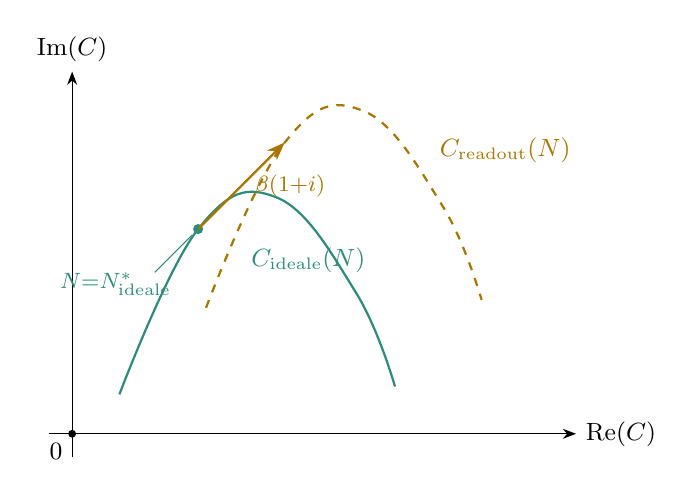
\begin{tikzpicture}[>=Stealth, font=\small]
 
  \draw[->] (-0.3,0) -- (6.4,0) node[right] {$\mathrm{Re}(C)$};
  \draw[->] (0,-0.3) -- (0,4.6) node[above] {$\mathrm{Im}(C)$};
  \filldraw[black] (0,0) circle (1.2pt) node[below left] {$0$};

 
  \draw[thick, teal2] plot[smooth, tension=0.7] coordinates
    {(0.6,0.5) (1.6,2.6) (2.6,3.0) (3.6,1.8) (4.1,0.6)};
  \filldraw[teal2] (1.6,2.6) circle (1.6pt);
  \node[teal2, font=\footnotesize] at (0.55,1.9) {$N{=}N^*_\text{ideale}$};
  \draw[teal2, thin] (1.05,2.05) -- (1.52,2.52);
  \node[teal2] at (3.0,2.2) {$C_\text{ideale}(N)$};

 
  \draw[->, amber!85!black, thick] (1.6,2.6) -- ++(1.1,1.1)
     node[midway, right=1pt, amber!85!black, font=\footnotesize] {$\beta(1{+}i)$};

 
  \draw[thick, amber!85!black, dashed] plot[smooth, tension=0.7] coordinates
    {(1.7,1.6) (2.7,3.7) (3.7,4.1) (4.7,2.9) (5.2,1.7)};
  \node[amber!85!black] at (5.5,3.6) {$C_\text{readout}(N)$};

\end{tikzpicture}
\caption{Effetto geometrico dell'Eq.~\eqref{eq:correlatore-affine} sul
luogo dei punti $C(N)$ nel piano complesso al variare di $N$ (curva
continua = ideale, $\alpha=1$ per semplicità del disegno). Il readout
simmetrico ($\beta=0$) lascerebbe la curva dove sta, cambiandone solo la
scala rispetto all'origine --- il punto più lontano dall'origine resta
il più lontano. Il readout asimmetrico ($\beta\neq0$) trasla l'\emph{intera}
curva di un vettore costante $\beta(1+i)$ (frecce arancioni, tutte
uguali): la distanza dall'origine di ciascun punto cambia in modo diverso
a seconda della sua posizione originaria, e il punto più lontano
dall'origine dopo la traslazione (massimo della curva tratteggiata) può
non essere più quello che lo era prima.}
\label{fig:traslazione-correlatore}
\end{figure}

\begin{center}
\fbox{\parbox{0.85\linewidth}{\centering
L'invarianza di $N^*$ è garantita solo se $\beta=0$ (readout simmetrico);
per $\beta\neq0$ non c'è nessuna garanzia analoga, va verificato
numericamente.}}
\end{center}

Questo è precisamente il tipo di affermazione che vale la pena
verificare con un conto: non un'estensione automatica di un risultato
già dimostrato, ma un'ipotesi che la teoria lascia esplicitamente aperta.
Se lo scarto $|\beta|$ è piccolo rispetto all'escursione di $|C_\text{ideale}(N)|$
lungo $N$, ci si aspetta che l'effetto sia piccolo (per continuità, un
$\beta\to0$ deve ridare il caso invariante); quanto piccolo debba essere
$|\beta|$ perché $N^*$ resti $5$ non è deducibile dalla sola
Eq.~\eqref{eq:correlatore-affine} senza sostituire numeri --- dipende
dalla forma specifica di $C_\text{ideale}(N)$ per il dimero, già nota
dai dati del Passo 4.

\section{Origine fisica dell'asimmetria}
\label{sec:origine-fisica}

Perché ci si aspetta $\beta\neq0$ su un hardware reale, e non solo per
completezza teorica? Il meccanismo dominante dell'errore di lettura nei
qubit superconduttori è il \textbf{rilassamento} ($T_1$) durante la
finestra di misura: un qubit preparato in $\ket1$ ha una probabilità non
nulla di decadere a $\ket0$ prima che la misura sia completata, mentre
non esiste un meccanismo altrettanto diretto per cui un qubit preparato
in $\ket0$ decada spontaneamente a $\ket1$ (violerebbe la conservazione
dell'energia in assenza di eccitazione esterna). Questo produce
un'asimmetria strutturale
\begin{equation}
p_{10} \;{\gtrsim}\; p_{01}
\end{equation}
osservata sistematicamente nelle proprietà di backend pubblicate da IBM
(\texttt{prob\_meas0\_prep1} $>$ \texttt{prob\_meas1\_prep0}, tipicamente
di un fattore $2$--$4\times$ su molti dispositivi Heron e precedenti) ---
coerente con il segno $\beta=p_{10}-p_{01}>0$ atteso.

\emph{Limite dichiarato esplicitamente}: la fonte già citata per la
calibrazione di riferimento (Stenger \emph{et al.}, arXiv:2504.15187)
riporta solo la mediana simmetrica $p_\text{readout}=2.3\times10^{-2}$,
non la scomposizione in $p_{01}$ e $p_{10}$ separati. Non è quindi
possibile, con la fonte già citata in tesi, ottenere uno split
asimmetrico \emph{realmente registrato per ibm\_torino}. La scelta dei
valori numerici per il test (Sez.~\ref{sec:verso-il-codice}) sarà quindi
dichiarata esplicitamente come \textbf{illustrativa} --- stesso trattamento
già riservato a $\varepsilon_{2q}$ nella nota di modellazione di
\texttt{noise\_model\_dimero.py} (``valore rappresentativo dell'ordine di
grandezza, non replica esatta dell'hardware'') --- coerente con
l'indicazione del relatore di non investire tempo eccessivo su questo
punto opzionale.

\section{Cosa non entra in questo modello}
\label{sec:cosa-non-entra-asimmetria}

Come per il Passo 1 (\texttt{teoria\_modello\_rumore.tex},
Sez.~``Cosa non entra''), è utile essere espliciti su cosa questa
estensione \emph{non} copre, per non lasciarlo implicito:
\begin{itemize}[leftmargin=1.3em,itemsep=0.2em]
\item \textbf{Correlazioni di lettura fra qubit} (crosstalk di misura): la
matrice di confusione dell'Eq.~\eqref{eq:confusione-asimmetrica} resta
per un singolo qubit (l'ancilla), applicata indipendentemente da quanto
succede sugli altri qubit --- coerente con l'uso di
\texttt{add\_all\_qubit\_readout\_error} nel resto della pipeline, qui
ristretto al solo qubit di misura del test di Hadamard.
\item $T_1$/$T_2$ restano esclusi come canali di evoluzione (decisione
del relatore, invariata): l'asimmetria discussa qui è solo
nell'\emph{atto di leggere} il risultato finale, non un modello di
rilassamento continuo durante il circuito.
\item Il readout resta applicato \textbf{analiticamente}
sull'aspettazione $\langle Z\rangle$ già calcolata con il rumore di gate,
non tramite un campionamento a shot finiti nel percorso principale ---
stessa scelta di tutta la pipeline. Il cross-check Monte Carlo con
\texttt{ReadoutError} vero (già usato nella verifica del caso simmetrico,
\texttt{validate\_correlatori\_rumorosi\_dimero.py}) va ripetuto con la
matrice asimmetrica dell'Eq.~\eqref{eq:confusione-asimmetrica} per la
stessa ragione: un secondo cammino di calcolo indipendente per lo stesso
risultato.
\end{itemize}

\section{Verso il codice}
\label{sec:verso-il-codice}

L'implementazione richiede due modifiche minime, entrambe localizzate:
\begin{itemize}[leftmargin=1.3em,itemsep=0.25em]
\item in \texttt{correlator\_rumoroso}, sostituire il singolo argomento
\texttt{p\_readout} con la coppia \texttt{(p01, p10)}, e la riga
\begin{quote}
\texttt{z\_re = ancilla\_z\_gate\_noisy(qc\_re, noise\_model) * (1 - 2 * p\_readout)}
\end{quote}
con l'applicazione diretta dell'Eq.~\eqref{eq:formula-generale},
\begin{quote}
\texttt{alpha = 1 - p01 - p10; beta = p10 - p01}\\
\texttt{z\_re = alpha * ancilla\_z\_gate\_noisy(qc\_re, noise\_model) + beta}
\end{quote}
(e identico per \texttt{z\_im}) --- la simmetria $p01=p10=p$ deve
riprodurre esattamente il ramo già in uso, primo controllo da fare;
\item per il cross-check Monte Carlo, costruire la
\texttt{ReadoutError} di Aer con la matrice
dell'Eq.~\eqref{eq:confusione-asimmetrica} al posto di quella simmetrica
--- Aer accetta direttamente una matrice di confusione non simmetrica,
nessuna estensione dell'API richiesta.
\end{itemize}
Il limite di rumore nullo ($p_{01}=p_{10}=0$) e il limite simmetrico
($p_{01}=p_{10}=p$, confrontato contro i risultati già registrati per
$N^*=5$) restano i primi due controlli obbligatori, nello stesso ordine
già seguito per ogni estensione della pipeline.

\section{Prossimo passo}

Applicare l'Eq.~\eqref{eq:formula-generale} con uno split $(p_{01},p_{10})$
esplicitamente dichiarato come illustrativo (Sez.~\ref{sec:origine-fisica}),
alla stessa griglia di $N$ già usata per il caso simmetrico, e verificare
se $N^*=5$ resta invariato o si sposta --- la domanda lasciata aperta dal
relatore, ora con una previsione teorica chiara su \emph{perché} potrebbe
non essere ovvio (Sez.~\ref{sec:rottura-invarianza}), non solo un numero
da ricontrollare.

\end{document}
